\subsubsection{Tables}

Pour créer des tables de résultats, j'ai lancé des campagnes de test avec des instances de trois tailles différentes : 500 noeuds, 1000 noeuds et la ville entière de Tours (44000 noeuds). Ces trois instances sont détaillées table \ref{tab:instances}. Ces instances sont des quartiers de Tours, qui m'ont été gentillement fournies par Félix Repusseau, un doctorant du LIFAT travaillant sur des problématiques similaires.

\begin{table}[!h]
\centering
\caption{Détail des instances utilisées. Pour le nombre de POI, le filtre est celui détaillé section \ref{sect:poi}.}
% \vspace{0.2cm}
\begin{tabular}{|c|c|c|c|c|}
\hline
Instance & Card(noeuds) & Card(arcs) & Card(POI) & Card(carreaux) \\  
\hline
$\texttt{500N\_0}$ & 498 & 1222 & 22 & 90 \\
\hline 
$\texttt{1000N\_0}$ & 1000 & 2517 & 41 & 235 \\
\hline 
$\texttt{Tours}$ & 43668 & 108431 & 3684 & 8831 \\
\hline 
\end{tabular}
\label{tab:instances}
\end{table}

L'objectif d'avoir plusieurs instances était de voir le comportement des algorithmes dans différents contextes, pour mieux couvrir les anomalies éventuelles, et d'avoir des résultats pour différentes tailles de graphe. Les modèles exacts sont très lents sur la métropole entière de Tours, pour pouvoir les comparer aux heuristiques sur des valeurs de paramètres (la distance maximale, le budget et le niveau LTS maximal) un peu réalistes, il fallait des instances plus petites. Les tables de résultats inclues dans ce rapport sont faites quasi exclusivement avec l'instance de 500 noeuds, parce que je n'ai pas constaté de différences significatives entre le comportement des différents modèles sur des tailles d'instances différentes.

J'ai fait des tests avec des paramètres non réalistes, juste pour avoir des résultats de comparaison de l'efficacité des modèles. J'ai aussi fait des tests avec des paramètres plus réalistes, pour voir ce qu'il se passait dans un cas proche d'une application réelle.

Les instances étant trop couteuses pour être lancées en local (Processeur Intel(R) Pentium(R) CPU 5405U @ 2.30GHz, 8 Go de mémoire RAM), mes tests ont été effectués sur le Mésocentre de Calcul CaSciModOT \cite{cas}. C'est un centre régional de calcul parallèle de taille intermédiaire entre des stations de travail et les grands centres nationaux (CINES, IDRIS, CCRT). Il permet de fournir à l'ensemble des partenaires de la fédération CaScIModOT une grappe possédant une puissance de calcul hautes performances. Les calculs sont lancés sur un processeur AMD Epyc 7702 à 2GHz.

\paragraph{Comparaison des algorithmes \ref{hpcc} et \ref{hpcc2} :}

La table \ref{tab:hdist2500} compare les algorithmes \ref{hpcc} et \ref{hpcc2} lorsque le tri effectué est le tri de \verb|pccs| dans l'ordre décroissant de la distance restante à aménager, elle donne des résultats similaires à l'heuristique où tout le budget. Appelons \verb|hdist2| la combinaison de ce tri et de l'algorithme \ref{hpcc2}, où l'on ne dépense pas tout le budget.

La valeur objective (OV) étant le critère \ref{criterepoi} de \ref{criteresopti}, plus le modèle est efficace, plus l'OV est faible.

La table se lit comme suit : ``sur la ligne 1, le jeu de données testé est \verb|500N_0|. Nous avons pris un budget de 1000 mètres, une distance maximale entre le point de départ et d'arrivée de 1400 mètres, et nous avons considéré comme sécurisées seulement les voies de facteur de danger inférieur à 1.2. Après optimisation, l'heuristique \verb|hdist| a atteint la valeur objective de 966 sur la visibilité des PCC, tout comme l'heuristique \verb|hdist2|. En comparaison, les valeurs objectives sur la visibilité exactes obtenues pour \verb|hdist| et \verb|hdist2| sont de 816. Le temps de calcul pris par \verb|hdist| est de 0.0109 secondes, et celui pris par \verb|hdist2| est de 0.01 secondes. Enfin, il restait 0.24 mètres de budget inutilisé avec \verb|hdist|, contre 15.39 mètres pour \verb|hdist2|, et ces heuristiques ont amélioré respectivement 39 et 38 arcs. ''

Nous constatons que les résultats entre les deux heuristiques sont similaires, et que le temps pris par les 2 heuristiques l'est aussi (la partie la plus coûteuse étant la construction des PCC). 

Cette table illustre notamment qu'il y a beaucoup de PCC entre un POI et un noeud délégué qui peuvent être complètement aménagés avec très peu de mètres, c'est à dire que les discontinuités dans le réseau cyclable (par exemple, des voies avec un danger très faible qui doivent traverser une route dangereuse à un croisement) jouent beaucoup à rendre le réseau non sécurisé. On améliorerait significativement le réseau en les supprimant.

Pour les restes des tests, des tables et des cartes, l'algorithme utilisé est toujours \ref{hpcc} (budget épuisé au maximum).

\paragraph{Ecart de valeur objective entre la visibilité exacte et la visibilité PCC :}

La table \ref{tab:nbppoi}, en annexe, illustre ce phénomène sur la fonction objective sur le nombre de POI atteints (le nombre de POI atteints - plus précisément, la somme sur les carreaux du nombre de POI qu'elles atteignent - valent le nombre de PPOI moins la valeur objective, puisque la valeur objective est le nombre de PPOI non atteints). Nous optimisons avec le modèle exact sur la visibilité PCC, puis nous comparons avant et après le nombre de POI atteints, en comptant cela avec les deux visibilités.

Cette table se lit de cette manière : ``sur la ligne 1, nous avons pris un budget de 1000 mètres, une distance maximale entre le point de départ et d'arrivée de 1400 mètres, et nous avons considéré comme sécurisées seulement les voies de danger inférieur à 1.2. Avant optimisation, 110 POI étaient atteints en les calculant avec la visibilité exacte, tandis que seulement 39 POI étaient atteints en les calculant avec la visibilité PCC. Après optimisation avec le modèle exact sur la visibilité PCC, on atteint 341 POI en les calculant avec la visibilité exacte, et 186 POI en les calculant avec la visibilité PCC.'' 

L'écart de valeur est proportionnel à l'augmentation du budget, de \verb|dmax| et du niveau LTS maximal. Nous remarquons que l'écart de nombre de POI atteints est important en fonction de la visibilité, même avant optimisation.

\paragraph{Comparaison de l'efficacité des différents modèles}

Nous pouvons comparer l'efficacité des modèles grâce aux tables \ref{tab:500ppoi}, \ref{tab:500popdist} et \ref{tab:500div}, se trouvant en annexe.

Pour ces tables, nous indiquons l'efficacité de chaque modèle, par erreur relative \cite{erreur_relative} sur les valeurs objectives (après optimisation). Plus exactement, nous calculons différentes erreurs relatives, données par :

\begin{enumerate}\label{enum:err}
    \item erreur relative, du point de vue de la visibilité PCC, du modèle exact sur la visibilité PCC par rapport à celle du modèle exact sur la visibilité exacte : $$100 \dfrac{(OV_{\text{exacte du modèle exact sur la visibilité PCC}} - OV_{\text{exacte du modèle exact sur la visibilité exacte}})}{OV_{\text{exacte du modèle exact sur la visibilité exacte}}},$$
    \item erreur relative, du point de vue de la visibilité PCC, d'une heuristique par rapport au modèle exact sur la visibilité PCC : $$100 \dfrac{(OV_{\text{PCC de l'heuristique}} - OV_{\text{PCC du modèle exact sur la visibilité PCC}})}{OV_{\text{PCC du modèle exact sur la visibilité PCC}}},$$
    \item erreur relative, du point de vue de la visibilité exacte, d'une heuristique par rapport au modèle exact sur la visibilité PCC : $$100 \dfrac{(OV_{\text{exacte de l'heuristique}} - OV_{\text{exacte du modèle exact sur la visibilité PCC}})}{OV_{\text{exacte du modèle exact sur la visibilité PCC}}}.$$
\end{enumerate}

Prenons la table \ref{tab:500ppoi}, elle se lit de cette manière : ``sur la ligne 2 de la table, nous avons pris un budget de 1000 mètres, une distance maximale entre le point de départ et d'arrivée (le point de départ étant le centre d'un carreau et le point d'arrivée un POI) de 500 mètres, et nous avons considéré comme sécurisées seulement les voies de danger inférieur à 1.2. L'algorithme exact a pris 137 secondes pour les calculs, l'algorithme exact sur une modélisation simplifiée a pris 0.4 secondes et l'algorithme heuristique a mis 0.0009 secondes. Pour ces paramètres, $$100 \dfrac{(OV_{\text{exacte du modèle exact sur la visibilité PCC}} - OV_{\text{exacte du modèle exact sur la visibilité exacte}})}{OV_{\text{exacte du modèle exact sur la visibilité exact}}}=13.483,$$
$$100 \dfrac{(OV_{\text{PCC de l'heuristique}} - OV_{\text{PCC du modèle exact sur la visibilité PCC}})}{OV_{\text{PCC du modèle exact sur la visibilité PCC}}}=8.85,$$
$$100 \dfrac{(OV_{\text{exacte de l'heuristique}} - OV_{\text{exacte du modèle exact sur la visibilité PCC}})}{OV_{\text{exacte du modèle exact sur la visibilité PCC}}}=11.881.''$$

Sur la ligne 1 de cette table, nous avons certaines colonnes vides, parce que le modèle exact sur la visibilité exacte n'a pas été calculé (le calcul prenant trop de temps ou de mémoire).

Il faut garder en tête que ces critères d'évaluation de l'efficacité des différents modèles sont imparfaits, puisqu'ils ne prennent pas en compte la valeur objective initiale, avant optimisation. Par exemple pour l'erreur relative n°1, si $OV_{\text{exacte du modèle exact sur la visibilité PCC}}=2$ et que $OV_{\text{exacte du modèle exact sur la visibilité exacte}}=1$, l'erreur relative est de 100\%. Si l'on suppose de plus qu'\emph{initialement}, $OV_{\text{exacte}}=11$, cela signifie que le modèle exact sur la visibilité PCC a trouvé 90\% des POI que le modèle exact sur la visibilité exacte a trouvé, ce qui n'est pas transmis par le 100\% d'erreur relative.

Les tables \ref{tab:500popdist} et \ref{tab:500div} se lisent de manière similaire. Pour la table \ref{tab:500div}, plus la valeur objective est grande, plus l'agorithme est efficace, donc la signification du signe de l'erreur relative est inversé. Pour les tables \ref{tab:500ppoi}, \ref{tab:500pop} et \ref{tab:500popdist} si l'erreur relative n°1 est positive, cela signifie que le modèle exact sur la visibilité exacte est meilleur que le modèle exact sur la visibilité PCC, alors que c'est l'inverse pour la table \ref{tab:500div}.

A partir de ces tables, nous pouvons faire une observation intéressante : la valeur objective des heuristiques, lorsqu'elle est calculée avec la visibilité des PCC, est, comme attendue, moins bonne que celle du modèle exact sur la visibilité PCC, puisque les heuristiques optimisent sur la même visibilité que le modèle exact sur la visibilité PCC (nous observons ça grâce à l'erreur relative n°2). En revanche, la valeur objective des heuristiques, lorsqu'elle est calculée avec la visibilité exacte, est parfois meilleure que celle du modèle exact sur la visibilité exacte (erreur relative n°3). Ce n'est pas absurde : c'est dû au fait que le modèle exact sur la visibilité des PCC est optimisé pour la visibilité des PCC, mais pas pour la visibilité exacte.

De plus, l'erreur n°2 est plus faible (en valeur absolue) pour le modèle sur la diversité, c'est possiblement parce qu'on a moins de choix de voies à aménager, puisqu'on réduit le nombre de POI sur lesquels on travaille.

La table \ref{tab:500div_detail} montre la répartition du nombre de catégories atteintes par les carreaux. Elle se lit de la manière suivante : ``prenons la seconde ligne, pour un budget de 1000 mètres, une distance maximale entre le point de départ et d'arrivée de 500 mètres, et considèrons comme sécurisées seulement les voies de danger inférieur à 1.2. En calculant cela avec la visibilité exacte, après optimisation avec le modèle exact sur la visibilité exacte, 44 carreaux ne peuvent pas atteindre de catégories, 13 carreaux peuvent atteindre une catégorie et 2 carreaux peuvent atteindre deux catégories. La logique est similaire pour les colonnes suivantes.''

Pour mettre les résultats dans leur contexte, pour \verb|dmax|=500, si le réseau était entièrement sécurisé, alors 43 carreaux ne pourraient toujours pas atteindre de catégories, 12 d'entre eux pourraient atteindre une catégorie au maximum et 4 d'entre eux pourraient atteindre deux catégories, et aucun carreau ne pourrait atteindre davantage de catégories. Pour \verb|dmax|=1400, alors un seul carreau ne pourrait toujours pas atteindre de catégories, 2 d'entre eux pourraient atteindre une catégorie au maximum et 56 d'entre eux pourraient atteindre deux catégories, et aucun carreau ne pourrait atteindre davantage de catégories.

Grâce à cette table, nous constatons que l'heuristique a en effet davantage tendance à effectuer des aménagements pour les carreaux ayant le moins de catégories atteintes, alors que les modèles exacts ne se soucient pas de cet aspect d'équité.

Pour des grandes valeurs de \verb|dmax|, nous ne pouvons pas faire fonctionner le modèle exact sur la visibilité exacte, donc nous pouvons seulement comparer les heuristiques avec le modèle exact sur la visibilité PCC. Nous pouvons néanmoins toujours calculer les valeurs objectives avec la visibilité exacte, pour les heuristiques et pour le modèle exact sur la visibilité exacte, même pour de grandes valeurs de \verb|dmax|. %, comme l'illustre la table \ref{tab:dmax_grand}.

% J'ai crée des tables plus détaillées, comparant plus de paramètres, que j'ai fourni à ma tutrice de stage. \textcolor{red}{mettre en annexe ?}

% Tester les modèles sur différentes tailles d'instances m'a permis de constater que l'efficacité des modèles ne varie pas avec la taille de l'instance, mais seulement avec la taille des paramètres (??).

\paragraph{Comparaison des heuristiques sur le critère d'optimisation \ref{criterepopu} de \ref{criteresopti} :}

Plusieurs heuristiques sur ce critère d'optimisation ont été testées. La table \ref{tab:compa_hpop} permet de les comparer, la meilleure heuristique sur chaque jeu de paramètre est mise en gras. L'heuristique imitant au mieux les performances du modèle exact sur la visibilité PCC est \verb|hpopdist| en général (l'erreur relative n°2 compare cela). Alors que l'heuristique \verb|hdist| est l'heuristique la moins bonne à cela, lorsqu'on recalcule sur la visibilité exacte les résultats des heuristiques, alors il arrive que ce soit cette heuristique qui donne les meilleurs résultats (l'erreur relative n°3 indique cela), bien que \verb|hpopdist| est aussi la meilleure en général.

\paragraph{Limites des modèles :}

Des valeurs réalistes de $\texttt{dmax}$ sont de 5 km (2 miles, la valeur utilisée dans \cite{kent_karner}), ou après échange avec Lou-Ann Deniau, 1,4 km, la distance moyenne qu'un cycliste effectue pour se rendre à un POI.

La plus grande distance $\texttt{dmax}$ que j'ai testée pour l'instance de Tours, avec le modèle exact sur la visibilité exacte, et pour les critères d'optimisation \ref{criterepoi} et \ref{criterepopu} de \ref{criteresopti}, est de 400 m. Au delà de cela, le calcul nécéssitait plus de 256 Go de mémoire, ou prenait plus de 24h. C'est éloigné des valeurs de $\texttt{dmax}$ sur lesquelles on souhaiterait que le modèle fonctionne.

Toujours pour les mêmes critères d'optimisation, pour l'instance de Tours, le modèle exact sur la visibilité PCC fonctionne sur \verb|dmax| = 1,4~km (plusieurs heures de calcul), mais pas sur \verb|dmax|~=~5~km.

Faute de temps, je n'ai pas pu quantifier précisément les limites des modèles exacts sur le critère sur la diversité de catégories de POI (\ref{criterecat} de \ref{criteresopti}). Les modèles exacts sur ce critère sont plus rapides, comme les tables de résultats permettent de le constater (il y a en effet moins de variables avec ce critère). Il est donc probable de pouvoir faire tourner ces modèles sur un paramètre \verb|dmax| légèrement supérieur, mais probablement pas 1,4 km pour le modèle exact sur la visibilité exacte.

Il est possible de faire tourner les heuristiques même sur de grands paramètres. Les tables permettent de constater que les heuristiques prennent toutes la même vitesse. Seules la valeur de \verb|dmax| et la taille de l'instance influencent la vitesse d'une heuristique, le niveau LTS et le budget maximal n'ont pas d'influence significative. Sur Tours et pour \verb|dmax|~=5~km, les heuristiques prennent environ 1h30 à calculer la solution.

\subsubsection{Cartes}

J'ai créé de multiples cartes, dont les objectifs étaient :

\begin{itemize}
    \item Voir visuellement les arcs à aménager pour diverses optimisations.
    \item Comparer les PM en fonction de différents paramètres.
    \item Comparer un PM avant-après une optimisation.
    \item Comparer les PM après différents modèles d'optimisation.
\end{itemize}

Les figures \ref{fig:carteinitiale}, \ref{fig:carteexacte}, \ref{fig:cartepcc} et \ref{fig:carteheuristique} montrent certains résultats trouvés pour la commune de Fondettes (voir figure \ref{figu:fondettes}), à proximité de Tours. Les PM sont calculés avec la visibilité exacte, pas avec la visibilité PCC. Pour ces cartes, la fonction objectif est la maximisation de différentes catégories de POI (critère \ref{criterecat} de \ref{criteresopti}), et les paramètres d'optimisation sont \verb|dmax| = 500 m, budget de 500 m de route à aménager et LTS maximale de 1.2. Les arcs à aménager trouvés par les différents modèles sont en rose. Le PM (calculé pour chaque carreau, en partant du noeud délégué) est ici : ``nombre de catégories accessibles en moins de 500 m par des voies de niveau LTS inférieur à 1.2''.

Nous constatons grâce à ces cartes ce que nous avons constaté grâce aux tables de résultats, par rapport à l'efficacité des différents modèles. Les cartes montrées ici ne sont pas exhaustives sur ce qu'elles permettent de visualiser, elles comparent juste les heuristiques pour une seule instance sur un seul jeu de données. Par exemple, il est pertinent d'observer ce qu'il se passe en augmentant le budget pour une optimisation, toutes choses égales par ailleurs, ou en augmentant \verb|dmax| ou le niveau LTS maximal.

Sur l'application, il est possible de zoomer, mais lorsqu'on enregistre une carte, on prend en fait un screenshot. On pert donc en qualité, et cela rend difficile la lecture d'une carte enregistrée représentant l'instance de Tours en entier, comme le montre la figure \ref{fig:cartetours}.

\begin{figure}[H]
    \centering
    \begin{subfigure}[t]{0.45\textwidth}
        \centering
        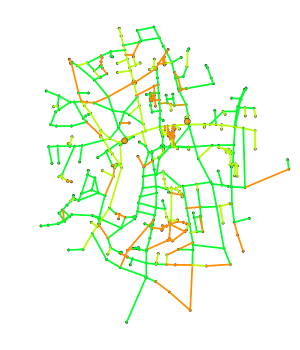
\includegraphics[width=\linewidth]{crop_500N_0.png}
        \caption{Carte initiale, le jeu de données est $\texttt{500N\_0}$. Les POI sur lesquels on optimise sont les points oranges.}
    \end{subfigure}
    \hfill
    \begin{subfigure}[t]{0.45\textwidth}
        \centering
        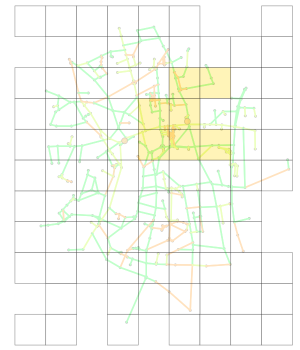
\includegraphics[width=\linewidth]{crop_500N_0_PM_Nombre_POI_accessibles_0,5km_LTS1,2.png}
        \caption{PM avant optimisation.}
    \end{subfigure}
    \caption{Situation initiale : carte et PM (nombre de catégories de POI accessibles à moins de 500 m avec un facteur LTS $\leq 1.2$).}
    \label{fig:carteinitiale}
\end{figure}

\begin{figure}[H]
    \centering
    \begin{subfigure}[t]{0.45\textwidth}
        \centering
        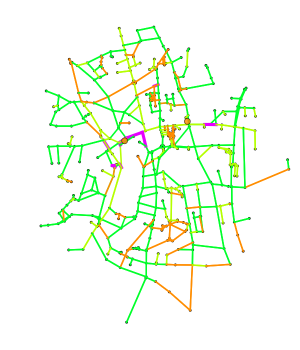
\includegraphics[width=\linewidth]{crop_500N_0_cplex_Budget_500_LTSmax_1.200_Dmax_500._cat_BA.png}
        \caption{Optimisation avec le modèle exact sur la visibilité exacte.}
    \end{subfigure}
    \hfill
    \begin{subfigure}[t]{0.45\textwidth}
        \centering
        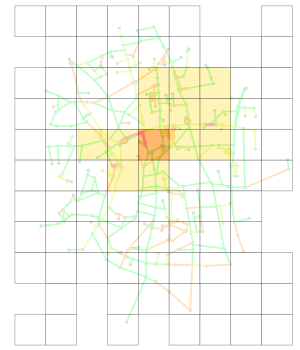
\includegraphics[width=\linewidth]{crop_500N_0_cplex_Budget_500_LTSmax_1.200_Dmax_500._cat_BA_PM_Nombre_POI_accessibles_0,5km_LTS1,2.png}
        \caption{PM après cette optimisation.}
    \end{subfigure}
    \caption{Optimisation avec le modèle exact sur la visibilité exacte : carte et PM associé.}
    \label{fig:carteexacte}
\end{figure}

\begin{figure}[H]
    \centering
    \begin{subfigure}[t]{0.45\textwidth}
        \centering
        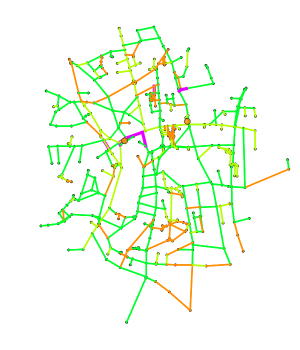
\includegraphics[width=\linewidth]{crop_500N_0_cplexvisi_Budget_500_LTSmax_1.200_Dmax_500._cat_BA.png}
        \caption{Optimisation avec le modèle exact sur la visibilité PCC.}
    \end{subfigure}
    \hfill
    \begin{subfigure}[t]{0.45\textwidth}
        \centering
        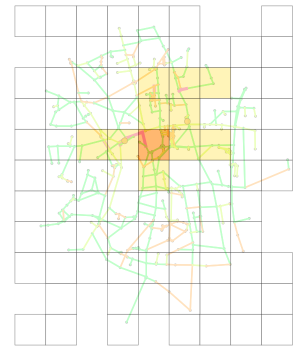
\includegraphics[width=\linewidth]{crop_500N_0_cplexvisi_Budget_500_LTSmax_1.200_Dmax_500._cat_BA_PM_Nombre_POI_accessibles_0,5km_LTS1,2.png}
        \caption{PM après cette optimisation.}
    \end{subfigure}
    \caption{Optimisation avec le modèle exact sur la visibilité PCC : carte et PM associé.}
    \label{fig:cartepcc}
\end{figure}

\begin{figure}[H]
    \centering
    \begin{subfigure}[t]{0.45\textwidth}
        \centering
        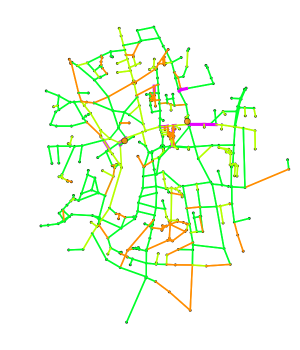
\includegraphics[width=\linewidth]{crop_500N_0_hdiversity_Budget_500_LTSmax_1.200_Dmax_500._BA.png}
        \caption{Optimisation avec heuristique sur la diversité de POI.}
    \end{subfigure}
    \hfill
    \begin{subfigure}[t]{0.45\textwidth}
        \centering
        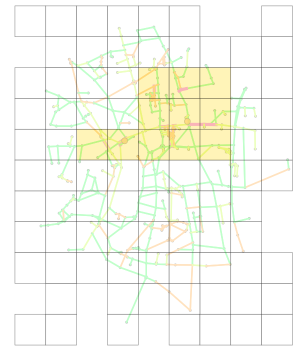
\includegraphics[width=\linewidth]{crop_500N_0_hdiversity_Budget_500_LTSmax_1.200_Dmax_500._BA_PM_Nombre_POI_accessibles_0,5km_LTS1,2.png}
        \caption{PM après cette optimisation.}
    \end{subfigure}
    \caption{Optimisation avec l'heuristique sur la diversité de catégories : carte et PM associé.}
    \label{fig:carteheuristique}
\end{figure}


% \begin{figure}[H]
%     \centering
%     \begin{subfigure}[t]{0.45\textwidth}
%         \centering
%         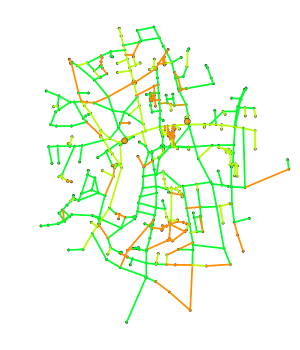
\includegraphics[width=1\linewidth]{crop_500N_0.png}
%         \caption{Carte initiale, le jeu de données est $\texttt{500N\_0}$. Les POI sur lesquels on optimise sont les points oranges.}
%     \end{subfigure}
%     \hfill
%     \begin{subfigure}[t]{0.45\textwidth}
%         \centering
%         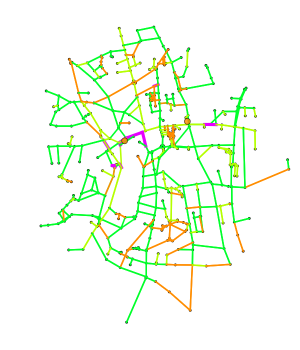
\includegraphics[width=1\linewidth]{crop_500N_0_cplex_Budget_500_LTSmax_1.200_Dmax_500._cat_BA.png}
%         \caption{Optimisation avec le modèle exact sur la visibilité exacte.}
%     \end{subfigure}
%     \hfill
%     \begin{subfigure}[t]{0.45\textwidth}
%         \centering
%         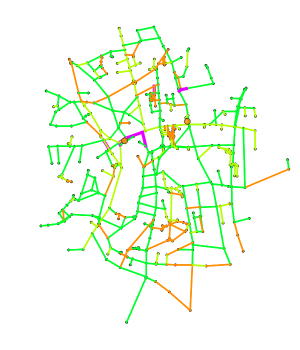
\includegraphics[width=1\linewidth]{crop_500N_0_cplexvisi_Budget_500_LTSmax_1.200_Dmax_500._cat_BA.png}
%         \caption{Optimisation avec le modèle exact sur la visibilité PCC.}
%     \end{subfigure}
%     \hfill
%     \begin{subfigure}[t]{0.45\textwidth}
%         \centering
%         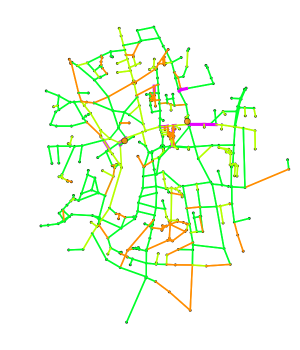
\includegraphics[width=1\linewidth]{crop_500N_0_hdiversity_Budget_500_LTSmax_1.200_Dmax_500._BA.png}
%         \caption{Carte obtenue avec l'heuristique sur la diversité de POI}
%     \end{subfigure}
%     \caption{Optimisation avec divers modèles, la fonction objectif est la maximisation de différentes catégories de POI (critère \ref{criterecat} de \ref{criteresopti}), et les paramètres d'optimisation sont $\texttt{dmax}$ = 500 m, budget de 500 m de route à aménager, LTS maximale de 1.2. Les arcs à aménager sont affichés en rose.}
%     \label{figu:arcs}
% \end{figure}

% \begin{figure}[H]
%     \centering
%     \begin{subfigure}[t]{0.45\textwidth}
%         \centering
%         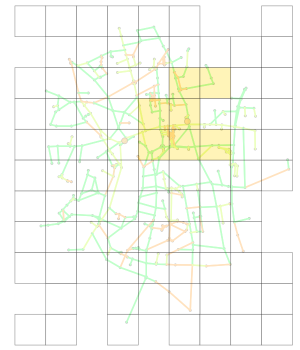
\includegraphics[width=1\linewidth]{crop_500N_0_PM_Nombre_POI_accessibles_0,5km_LTS1,2.png}
%         \caption{PM avant optimisation}
%     \end{subfigure}
%     \hfill
%     \begin{subfigure}[t]{0.45\textwidth}
%         \centering
%         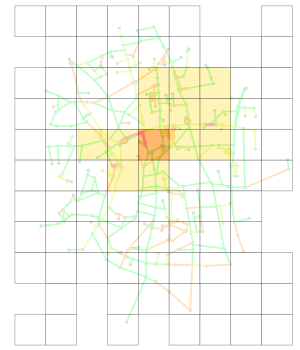
\includegraphics[width=1\linewidth]{crop_500N_0_cplex_Budget_500_LTSmax_1.200_Dmax_500._cat_BA_PM_Nombre_POI_accessibles_0,5km_LTS1,2.png}
%         \caption{PM après optimisation avec le modèle exact sur la visibilité exacte.}
%     \end{subfigure}
%     \hfill
%     \begin{subfigure}[t]{0.45\textwidth}
%         \centering
%         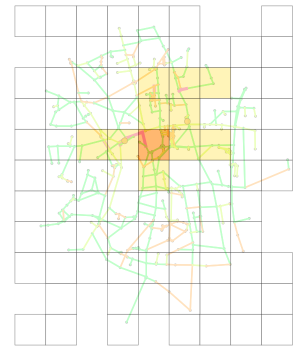
\includegraphics[width=1\linewidth]{crop_500N_0_cplexvisi_Budget_500_LTSmax_1.200_Dmax_500._cat_BA_PM_Nombre_POI_accessibles_0,5km_LTS1,2.png}
%         \caption{PM après optimisation avec le modèle exact sur la visibilité PCC.}
%     \end{subfigure}
%     \hfill
%     \begin{subfigure}[t]{0.45\textwidth}
%         \centering
%         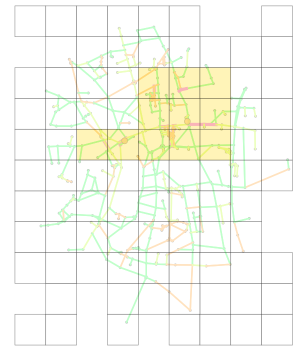
\includegraphics[width=1\linewidth]{crop_500N_0_hdiversity_Budget_500_LTSmax_1.200_Dmax_500._BA_PM_Nombre_POI_accessibles_0,5km_LTS1,2.png}
%         \caption{PM après optimisation avec l'heuristique sur la diversité de catégories de POI.}
%     \end{subfigure}
%     \caption{PM avant et après optimisation avec divers modèles, appliqués aux optimisation représentées précédemment. Le PM est le suivant : nombre de catégories accessibles en moins de 500 m par des voies de niveau LTS inférieur à 1.2. En jaune, les carreaux atteignants une catégorie de POI, en orange, les carreaux en atteignant deux.}
%     \label{figu:pm}
% \end{figure}

\begin{figure}[H]
    \centering
    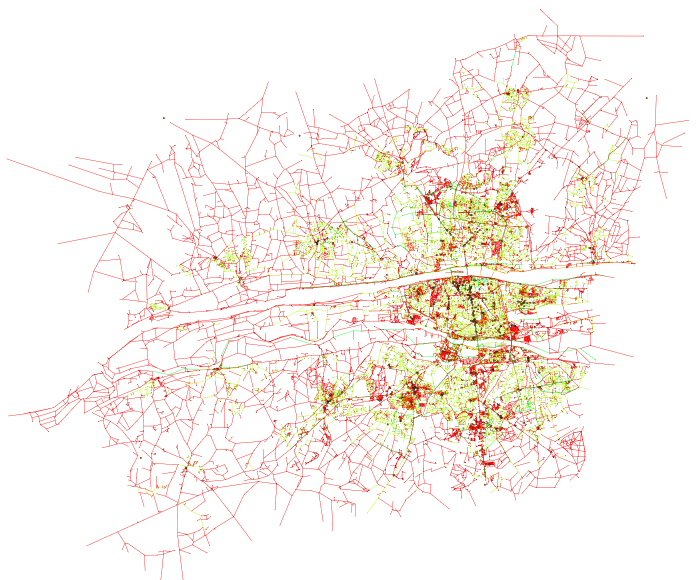
\includegraphics[width=1\linewidth]{crop_Tours_hdiversity_Budget_2000_LTSmax_1.200_Dmax_5000_BA.png}
    \caption{Carte de l'instance de Tours, après optimisation avec les paramètres $\texttt{dmax}~=~5~km$, budget de 2 km, et LTS $\leq 1.2$. Difficile de repérer les arcs à aménager, ce qui n'est pas idéal pour communiquer avec les cartographes.}
    \label{fig:cartetours}
\end{figure}


\subsection{Difficultés rencontrées}\label{sect:diff}

\paragraph{Déboguage :}

Une des difficultés majeures de ce stage a été le déboguage des modèles et des fonctions. Pour avoir des résultats intéressants, il faut un graphe d'au moins 100 noeuds. Il est donc nécessaire d'avoir des instances de test, pour vérifier que les fonctions ont bien le comportement attendu.

Un problème se pose, il est difficile d'être exhaustif sur tous les cas particuliers pouvant créer des erreurs lorsqu'on crée une instance de test.

Ainsi, j'avais des erreurs qui apparaissaient seulement dans des grands graphes, pour lesquels faire tourner l'algorithme à la main est fastidieux et difficile. J'ai néanmoins dû me rabattre sur cette méthode pour déboguer certaines erreurs, mes instances tests me servaient seulement à vérifier le comportement de mes fonctions lors du développement. Lorsque je repérais un bug sur une instance précise, je lançais le débogueur C++ jusqu'à trouver l'erreur.

Déboguer les modèles CPLEX est aussi difficile, de manière générale. Le fichier \verb|.lp| généré, permettant de voir les variables et contraintes crées par CPLEX, fait déjà plusieurs centaines de lignes pour un graphe d'une dizaine de noeuds.


\paragraph{Arrondir le facteur de danger pour des raisons de cohérence :}

Les données qui m'étaient fournies pour calculer le niveau LTS sur un tronçon étaient deux nombres, la distance en mètres du tronçon et un nombre "danger", dont le ratio $\fFrac{\text{danger}}{\text{distance}}$ était censé appartenir à l'ensemble $R=\{1; 1.15; 1.3; 1.375; 1.45; 1.75\}$. Ces données étaient stockées dans le fichier \verb|.csv| des arcs du réseau.

Il arrivait que ce ratio soit légèrement supérieur à l'une de ces valeurs, par exemple $1.3+10^{-8}$. Lors des applications réelles de ce programme, intuitivement, on veut optimiser en fournissant un ratio maximum appartenant à $R$. Cela pose alors problème, parce qu'un arc ayant un ratio très légèrement supérieur à une valeur de $R$ sera traité comme étant à aménager, alors qu'il s'agit juste d'un problème d'arrondi et qu'on le considère déjà comme empruntable.

J'ai donc essayé d'ajouté une tolérance lors de l'optimisation, pour que les arcs légèrement supérieurs à une valeur $v$ de l'ensemble $R$ soient traités comme s'ils étaient à $v$. En plus du problème de cohérence avec les applications réelles, l'absence de tolérance posait un problème de cohérence entre les deux projets : les arrondis du facteur LTS, décrit au paragraphe précédent, n'étaient pas les mêmes sur les deux projets, le facteur étant enregistré sous forme de double dans Bike Accessibility, et sous forme de float dans Chemins Equitables.

Je n'ai néanmoins pas eu le temps de bien tout tester de nouveau, je ne peux pas être certain que tout fonctionne correctement.

\paragraph{Travailler sur deux projets :}

J'ai repris deux projets déjà entamés par le LIFAT, Bike Accessibility (optimisation d'un réseau cyclable) et Chemins Equitables (visualisation d'indicateurs d'équités). J'ai ensuite dû faire communiquer ces deux projets. 

Dans les projets Bike Accessibility et Chemins Equitables, des étapes se succédaient entre ces deux projets, voir parfois certaines étapes étaient effectuées sur les 2 projets à la fois (par exemple, le calcul des PM est implicitement fait sur le projet Bike Accessibility, puisque on calcule déjà la possibilité d'emprunter chaque chemin, et un autre exemple étant la gestion du facteur LTS, détaillé au paragraphe précédent). Il fallait alors s'assurer de la cohérence des résultats trouvés sur chacun de ces projets. 

Mon objectif a été de faire mes modifications au maximum sur le projet Bike Accessibility, pour réduire le risque d'erreur entre la communication entre les projets. C'est cette logique qui m'a poussé, pour l'optimisation sur la diversité de catégories de POI, j'ai choisi de filtrer les POI dans le parser de Bike Accessibility, plutôt que de générer un nouveau fichier POI dans l'application Chemins Equitables et d'utiliser celui là (l'autre avantage étant de pouvoir faire l'optimisation sur le même jeu de données directement). Mon objectif était ensuite de générer sur Bike Accessibility un nouveau fichier POI contenant seulement les POI sur lesquels l'optimisation a été faite (ceux d'une des catégories conservées).

L'idéal aurait été de tout générer dans le projet Bike Accessibility, pour réduire le risque d'erreur à cause d'incohérences. Or, insérer toute la partie génération de données post-optimisation, ainsi que la partie génération de PM avant et après optimisation, dans le projet Bike Accessibility, de manière propre et facilement expandable si l'on rajoute des modèles, était une tâche compliquée. Pour référence, le développement de toutes ces étapes sur l'application Chemins Equitables a été faite en 2 mois par deux stagiaires à la fois.

Ma solution a été de vérifier à la main la cohérence des deux projets, et d'ajouter des fonctions de test à certains endroits. Par exemple, sur la figure \ref{fig:nb_poi_compa}, on peut voir une comparaison visuelle des résultats de ces deux projets, pour le nombre de POI accessibles par chaque carreaux.

\begin{figure}[H]
\centering
    \begin{tabular}{cc}    
        \begin{minipage}[t]{2.5in}
        \centering
        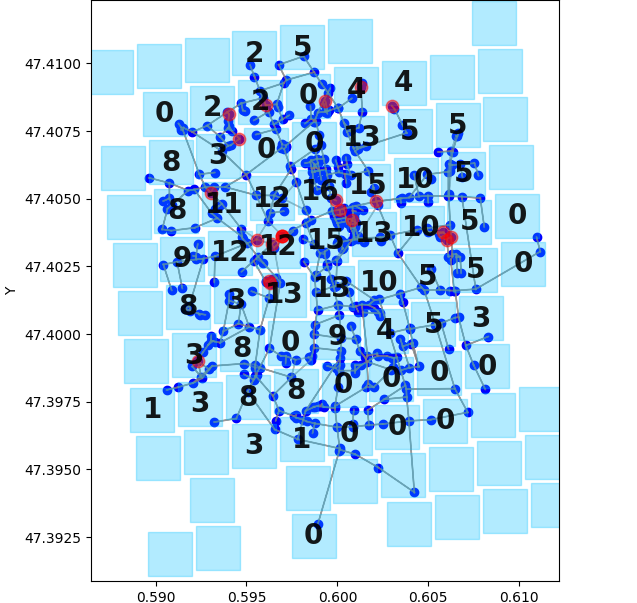
\includegraphics[height=2in]{nb_poi_BA.png}
        % \label{fig:task1_l1}
        \end{minipage}
    %%    
        \begin{minipage}[t]{2.5in}
        \centering
        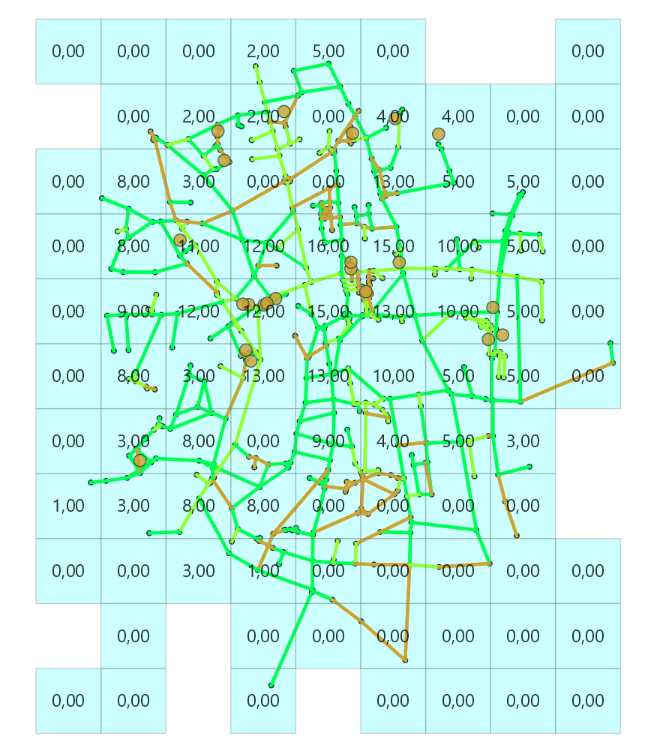
\includegraphics[height=2in]{nb_poi_CE.png}
        % \label{fig:task1_cpu}
        \end{minipage}
    \end{tabular}
    \caption{Un des tests pour vérifier la cohérence des deux projets. A gauche, le nombre de POI accessibles par carreau INSEE pour le projet Bike Accessibility. A droite, le nombre de POI accessibles par carreau INSEE pour le projet Chemins Equitables. Pour la ville de Fondettes, dans l'agglomération de Tours.}
    \label{fig:nb_poi_compa}
\end{figure}

J'ai codé dans le projet Bike Accessibility la génération d'un PM (pour l'heuristique sur la diversité de catégories), et j'ai comparé les résultats donnés avec le même PM codé sur l'application Chemins Equitables. En revanche, on ne peut pas être certain d'être exhaustif en vérifiant complètement seulement certains éléments.

Quant aux POI, j'ai fini par coder un filtre pour afficher seulement les POI pertinents sur les cartes, pour avoir des cartes exploitables par les cartographes (mais utiliser ce fichier POI nécéssitait de modifier des choses à la main, alors que ces étapes sont automatisées sinon. En somme, ce n'est pas une solution idéale).
